%! Author = tstreule

\section{Biosensors}
%%%%%%%%%%%%%%%%%%%%%%%%%%%%%%%%%%%%%%%%%%%%%%%%%%%%%%
%%%%%%%%%%%%%%%%%%%%%%%%%%%%%%%%%%%%%%%%%%%%%%%%%%%%%%
%	\subsection{Biosensors Principle}
%	%
%	\begin{center}
%		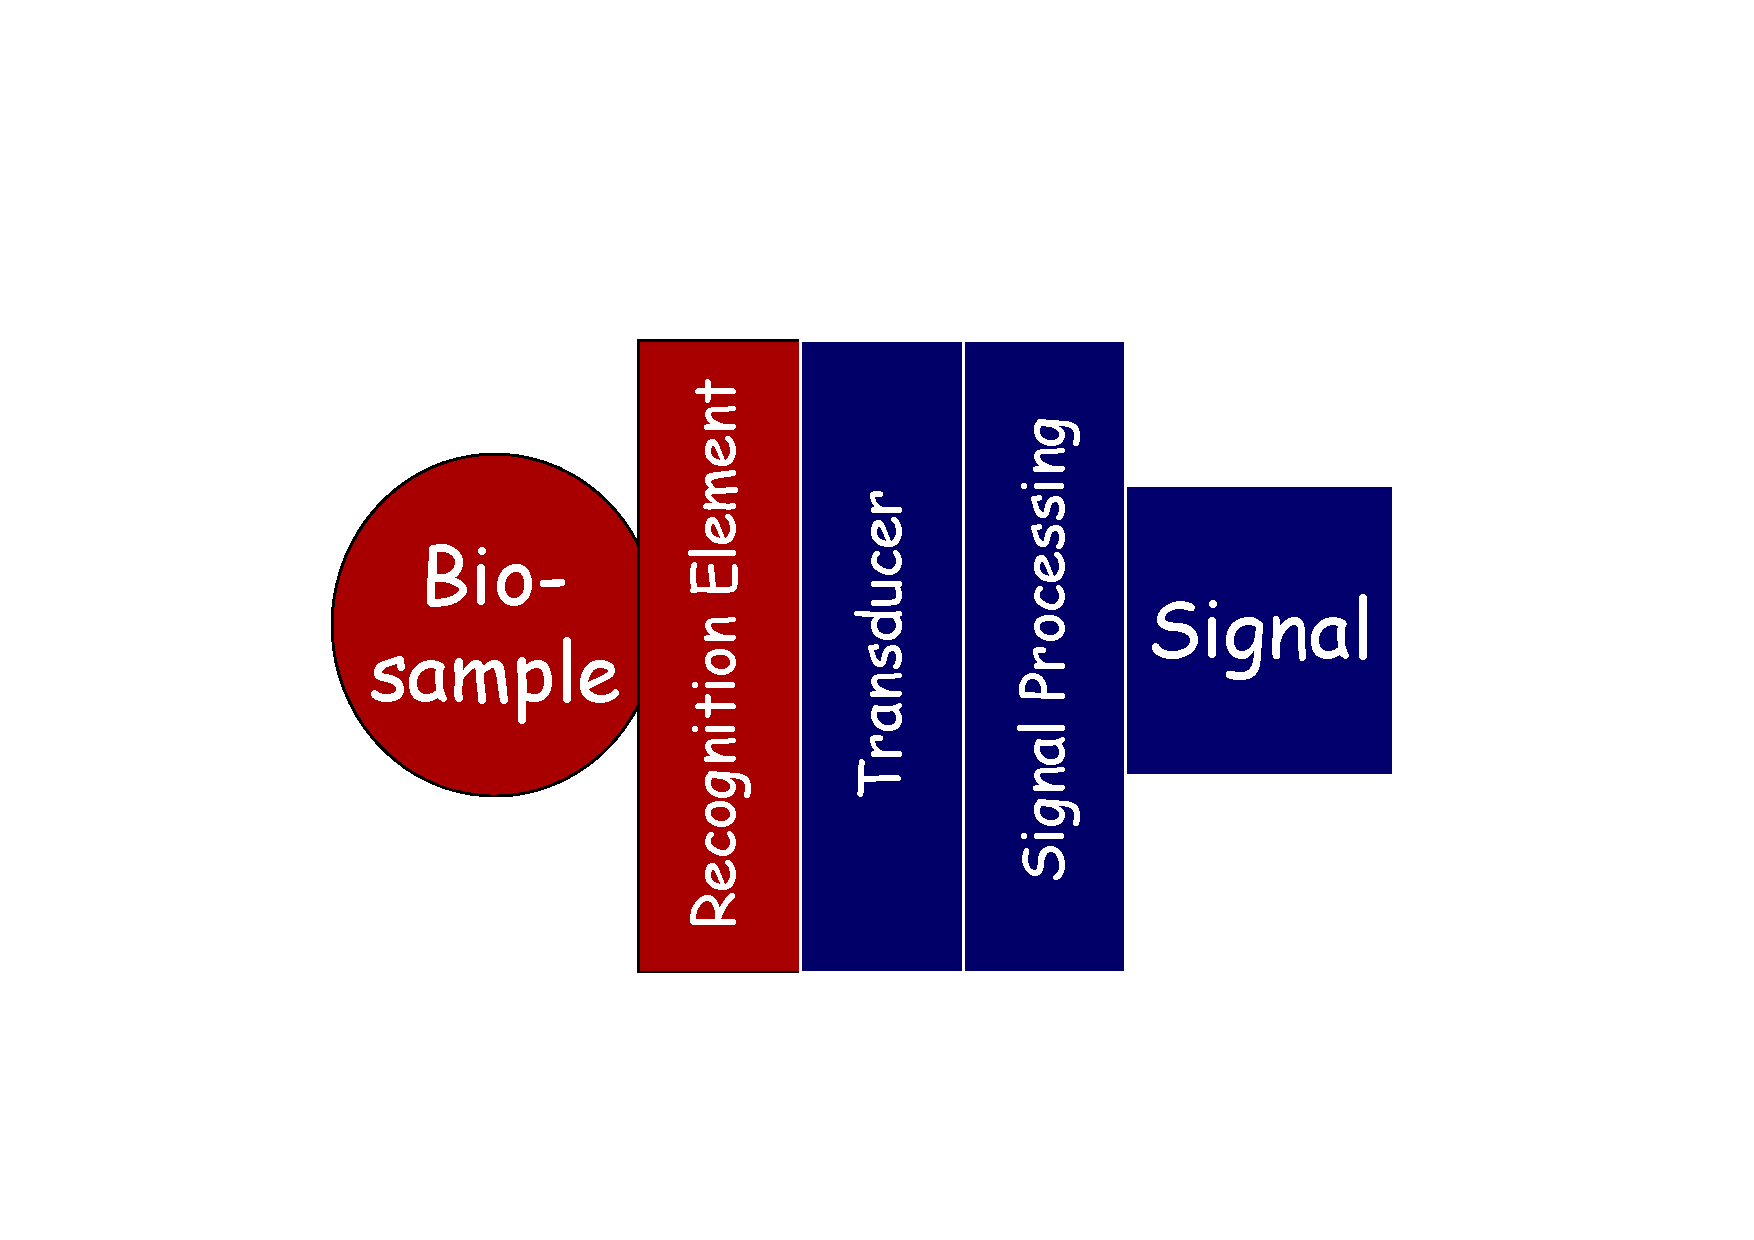
\includegraphics[width=.3\columnwidth]{Biosensors_Principle}
%	\end{center}
%%%%%%%%%%%%%%%%%%%%%%%%%%%%%%%%%%%%%%%%%%%%%%%%%%%%%%
\subsection{Label assay vs. label-free}
%
\shortstack{Label assay\\(sandwich):}
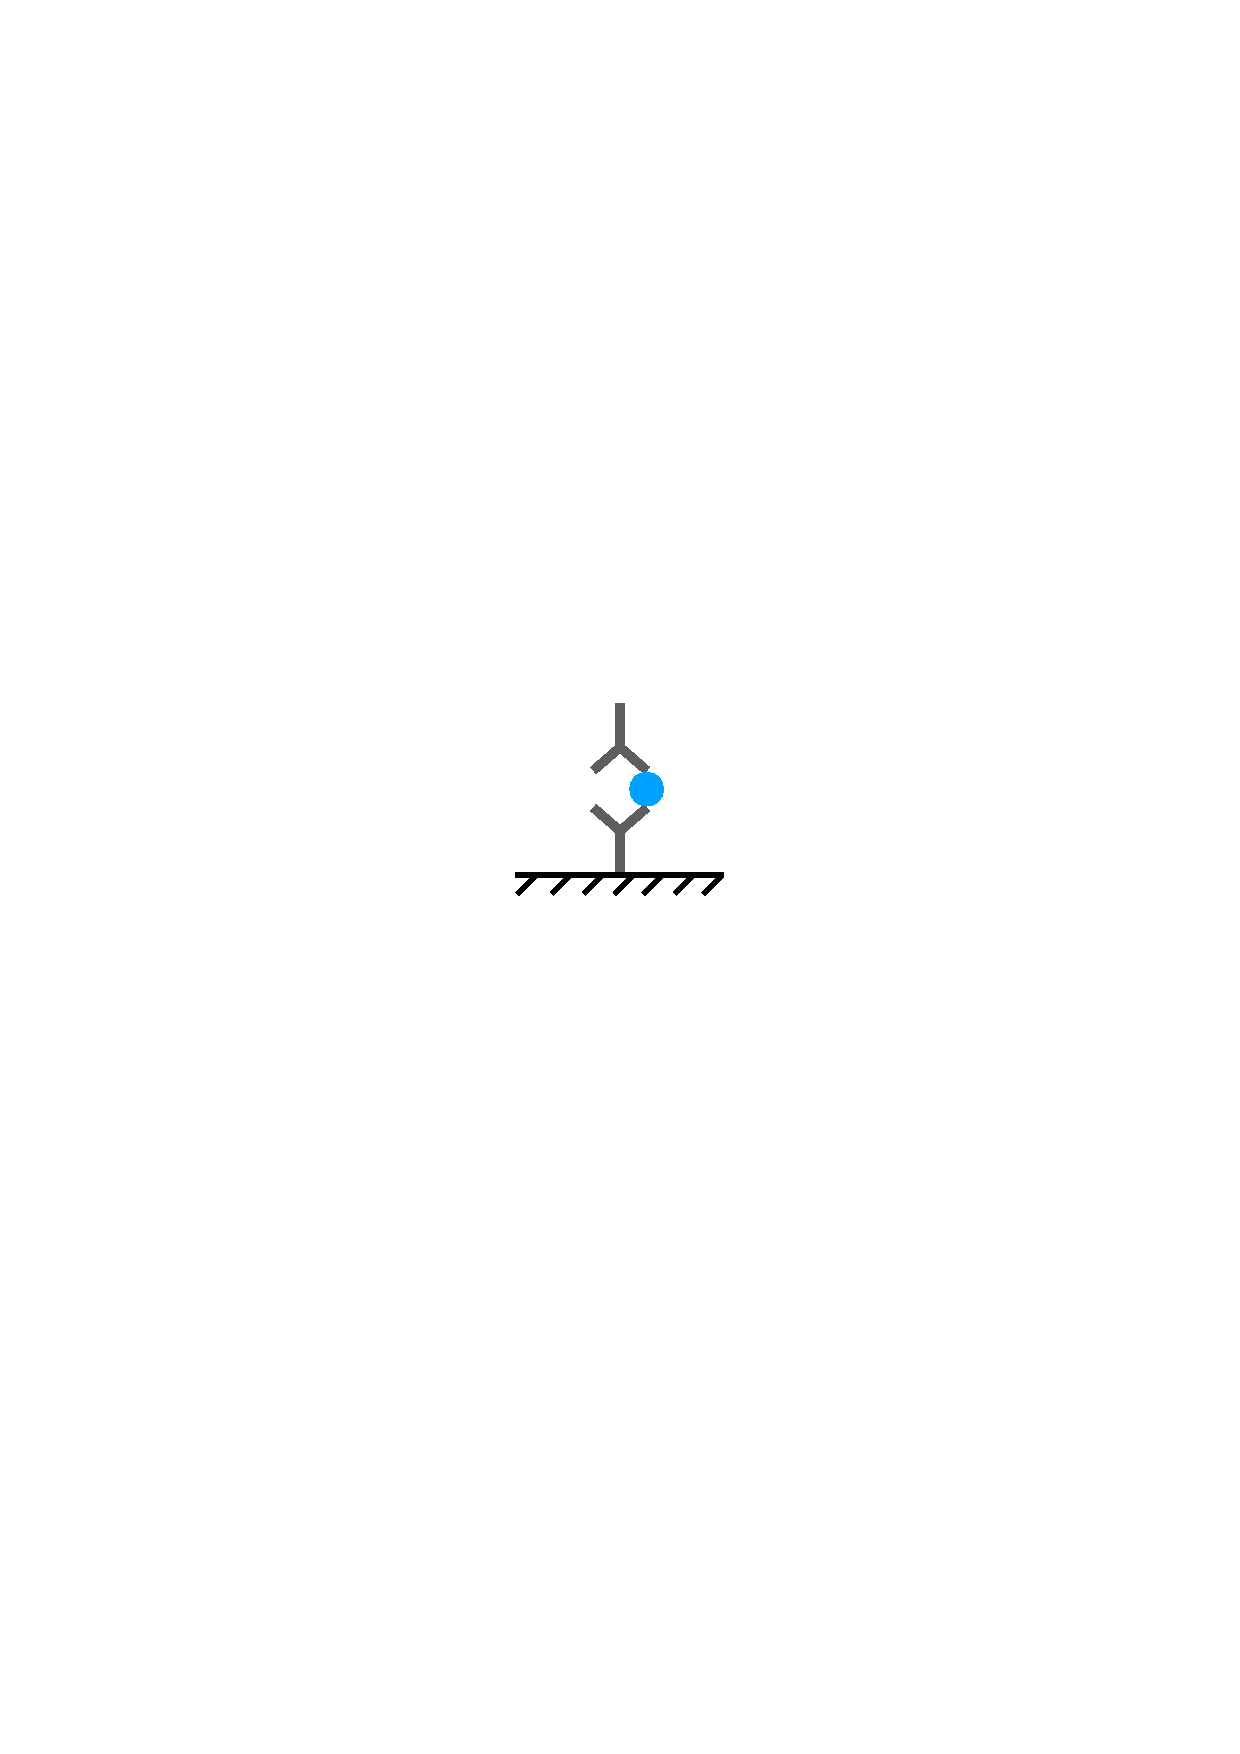
\includegraphics[width=.08\columnwidth]{Biosensors_Label_Assay}
\qquad
\shortstack{Label-free assay\\(OWLS):}
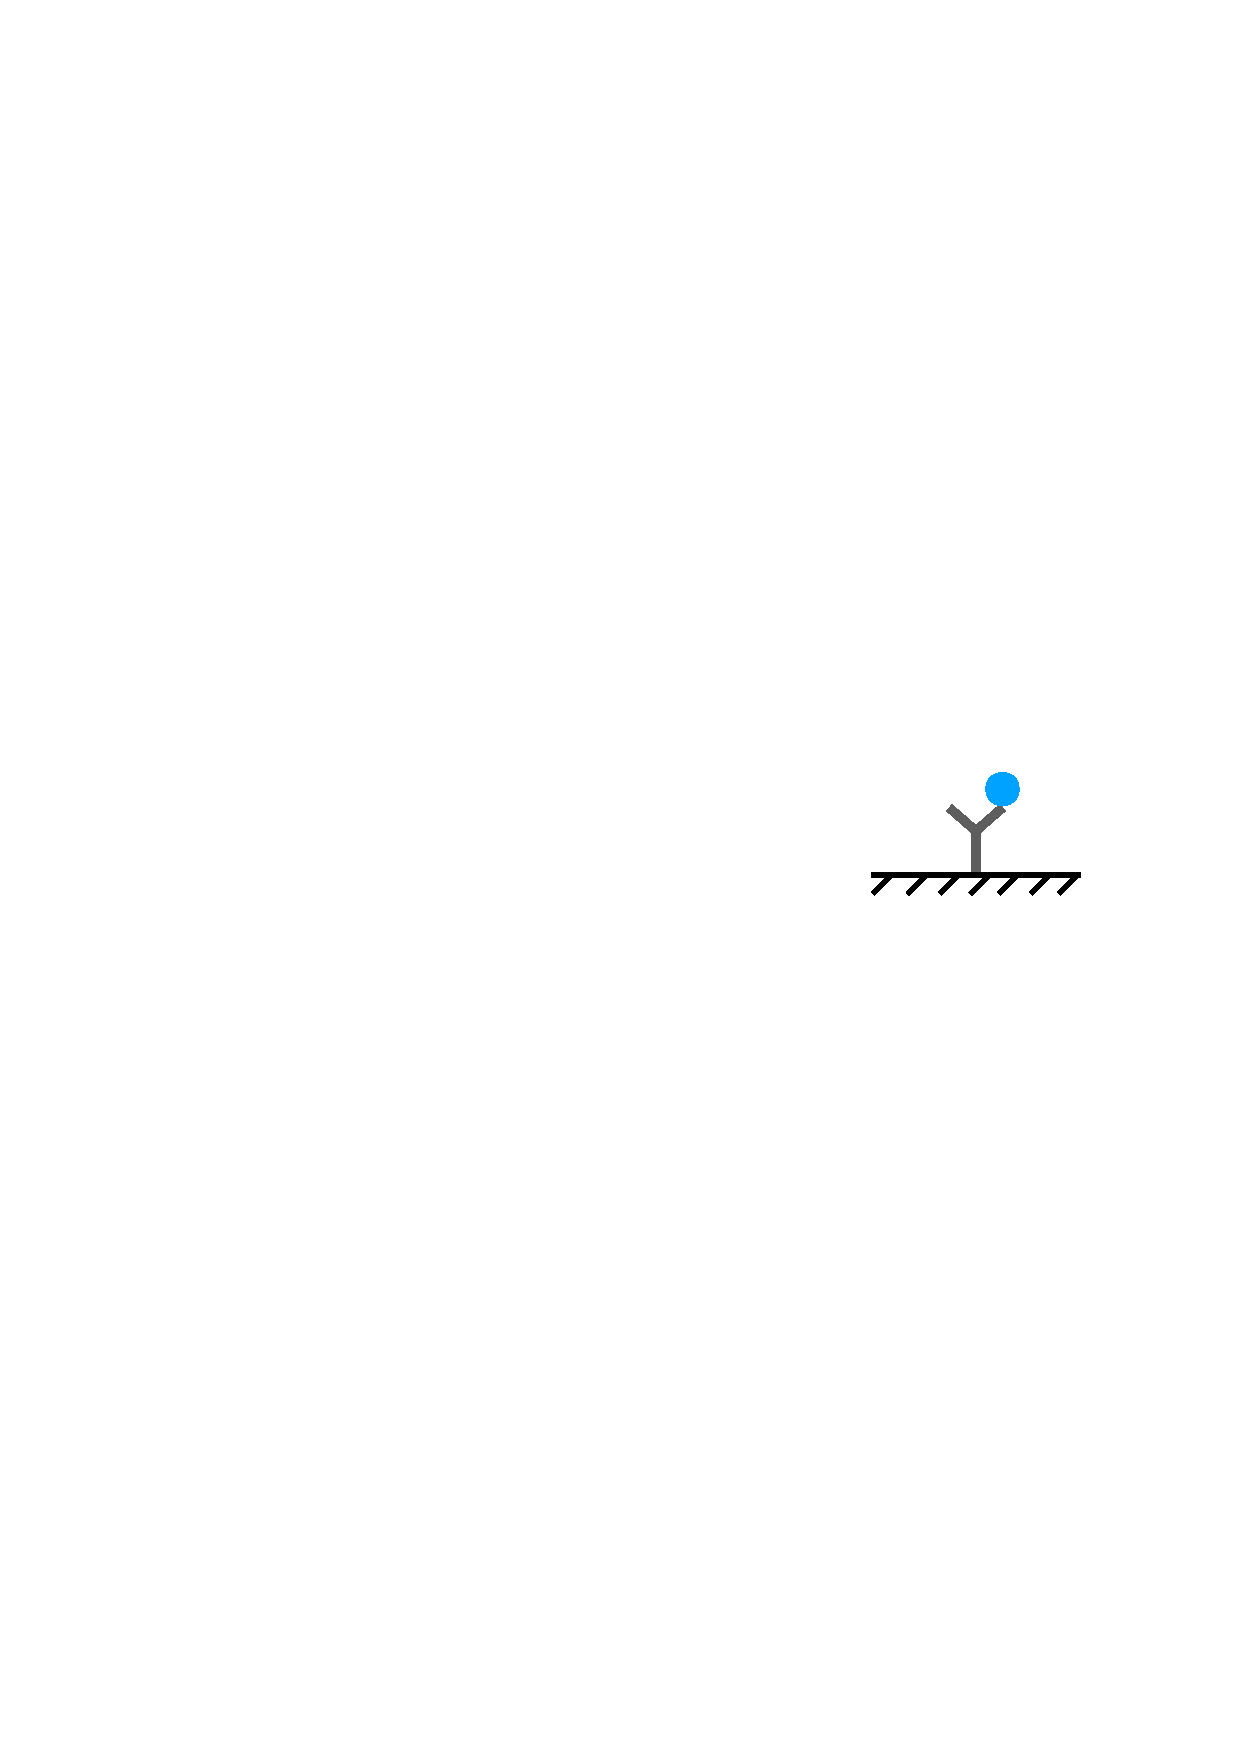
\includegraphics[width=.08\columnwidth]{Biosensors_Label_Free}
\par
\shortstack{non-specific\\binding:}
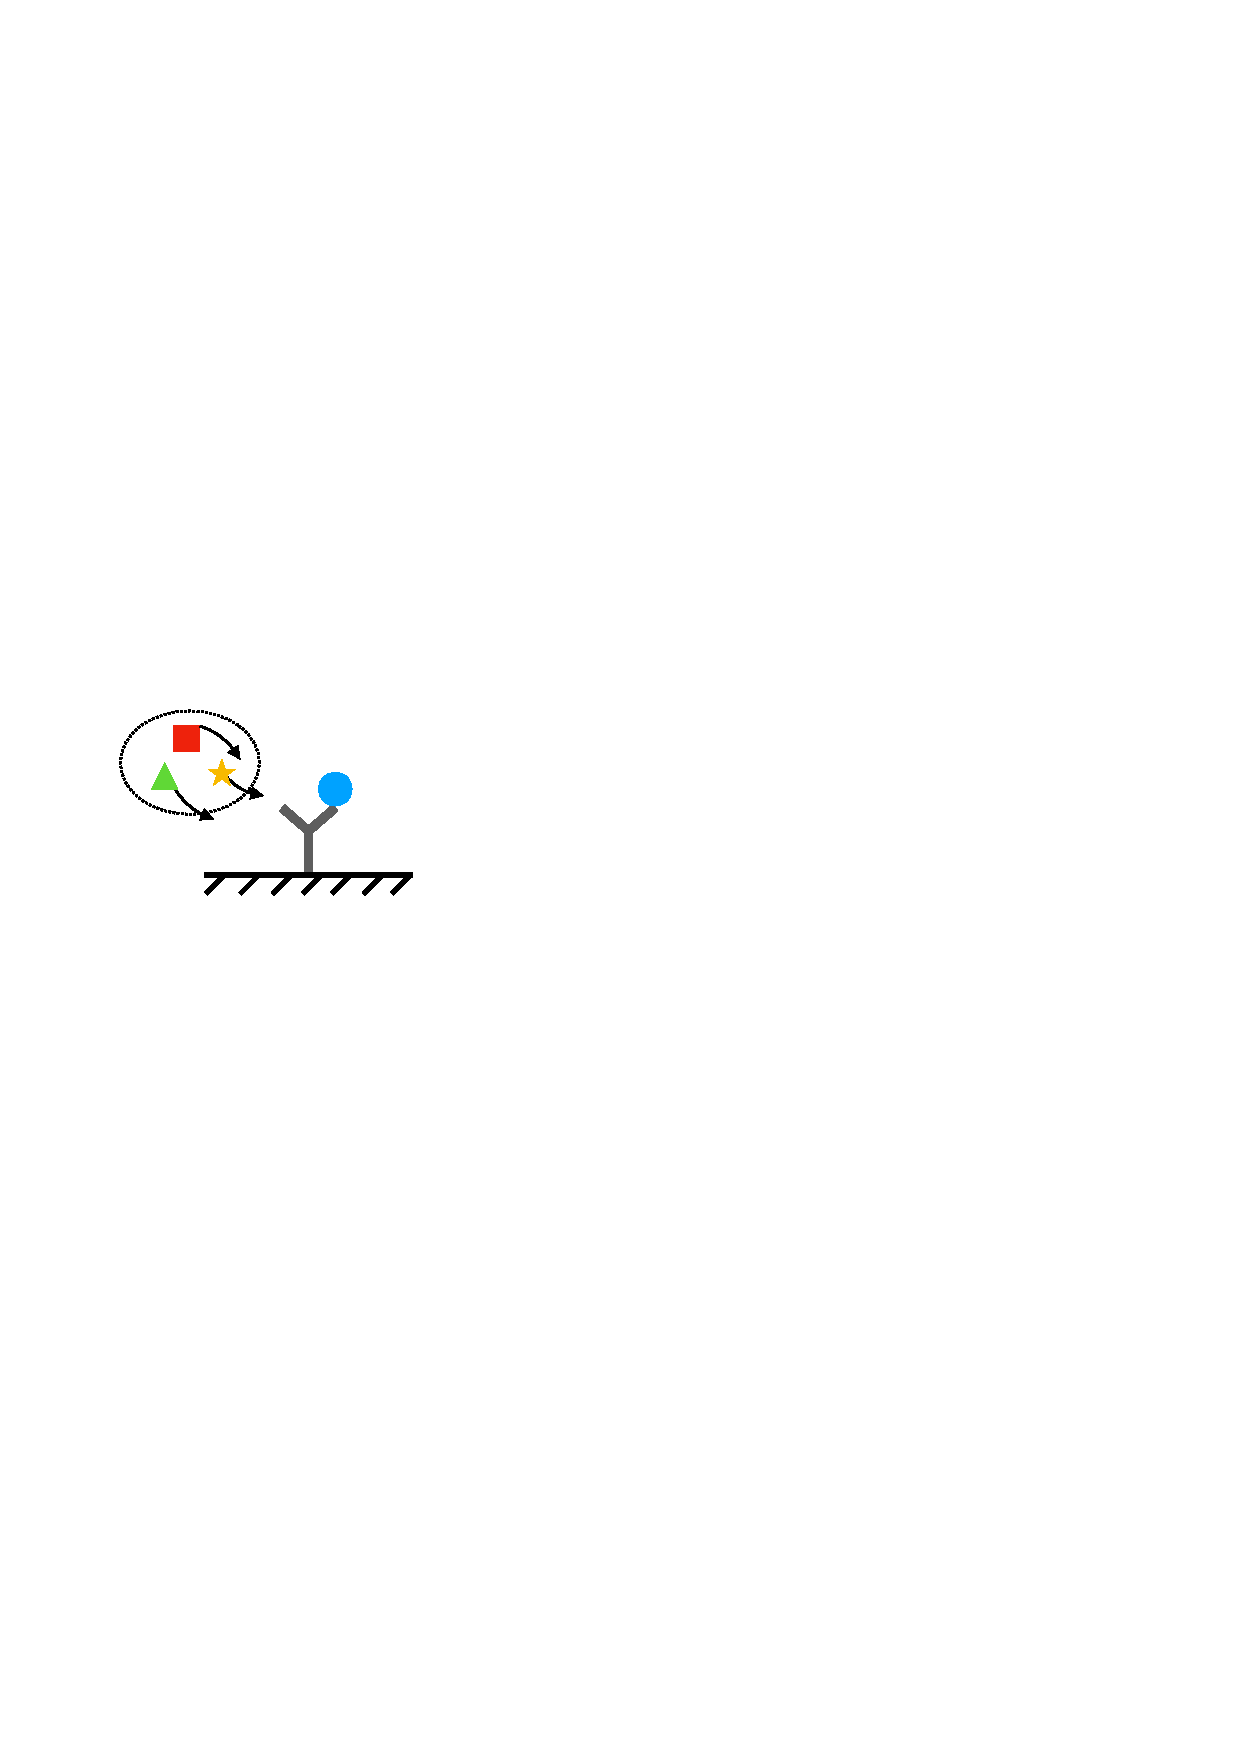
\includegraphics[width=.12\columnwidth]{Biosensors_Non_Specific}
\shortstack[r]{other interactions that could happen,\\ except the angle binding.}
%%%%%%%%%%%%%%%%%%%%%%%%%%%%%%%%%%%%%%%%%%%%%%%%%%%%%%
\subsection{Rules of Chemistry and Physics}
%
\formtex{\textit{Bracket notation}}{indicates concentration}
\ce{A +B <=>[$k_1$][$k_{-1}$] AR}
\formbox{equilibrium constant}{K = \frac{k_{-\!1}}{k_1} = \frac{[A][R]}{[AR]}}
\formula{affinity constant}{K_a = 1/K}
\formula{cont. flowing cell}{[AR] \sim q * \text{signal},}
$q=const$
\formula{~}{[R] \sim R_0 = \text{initial receptor density}}
%
%	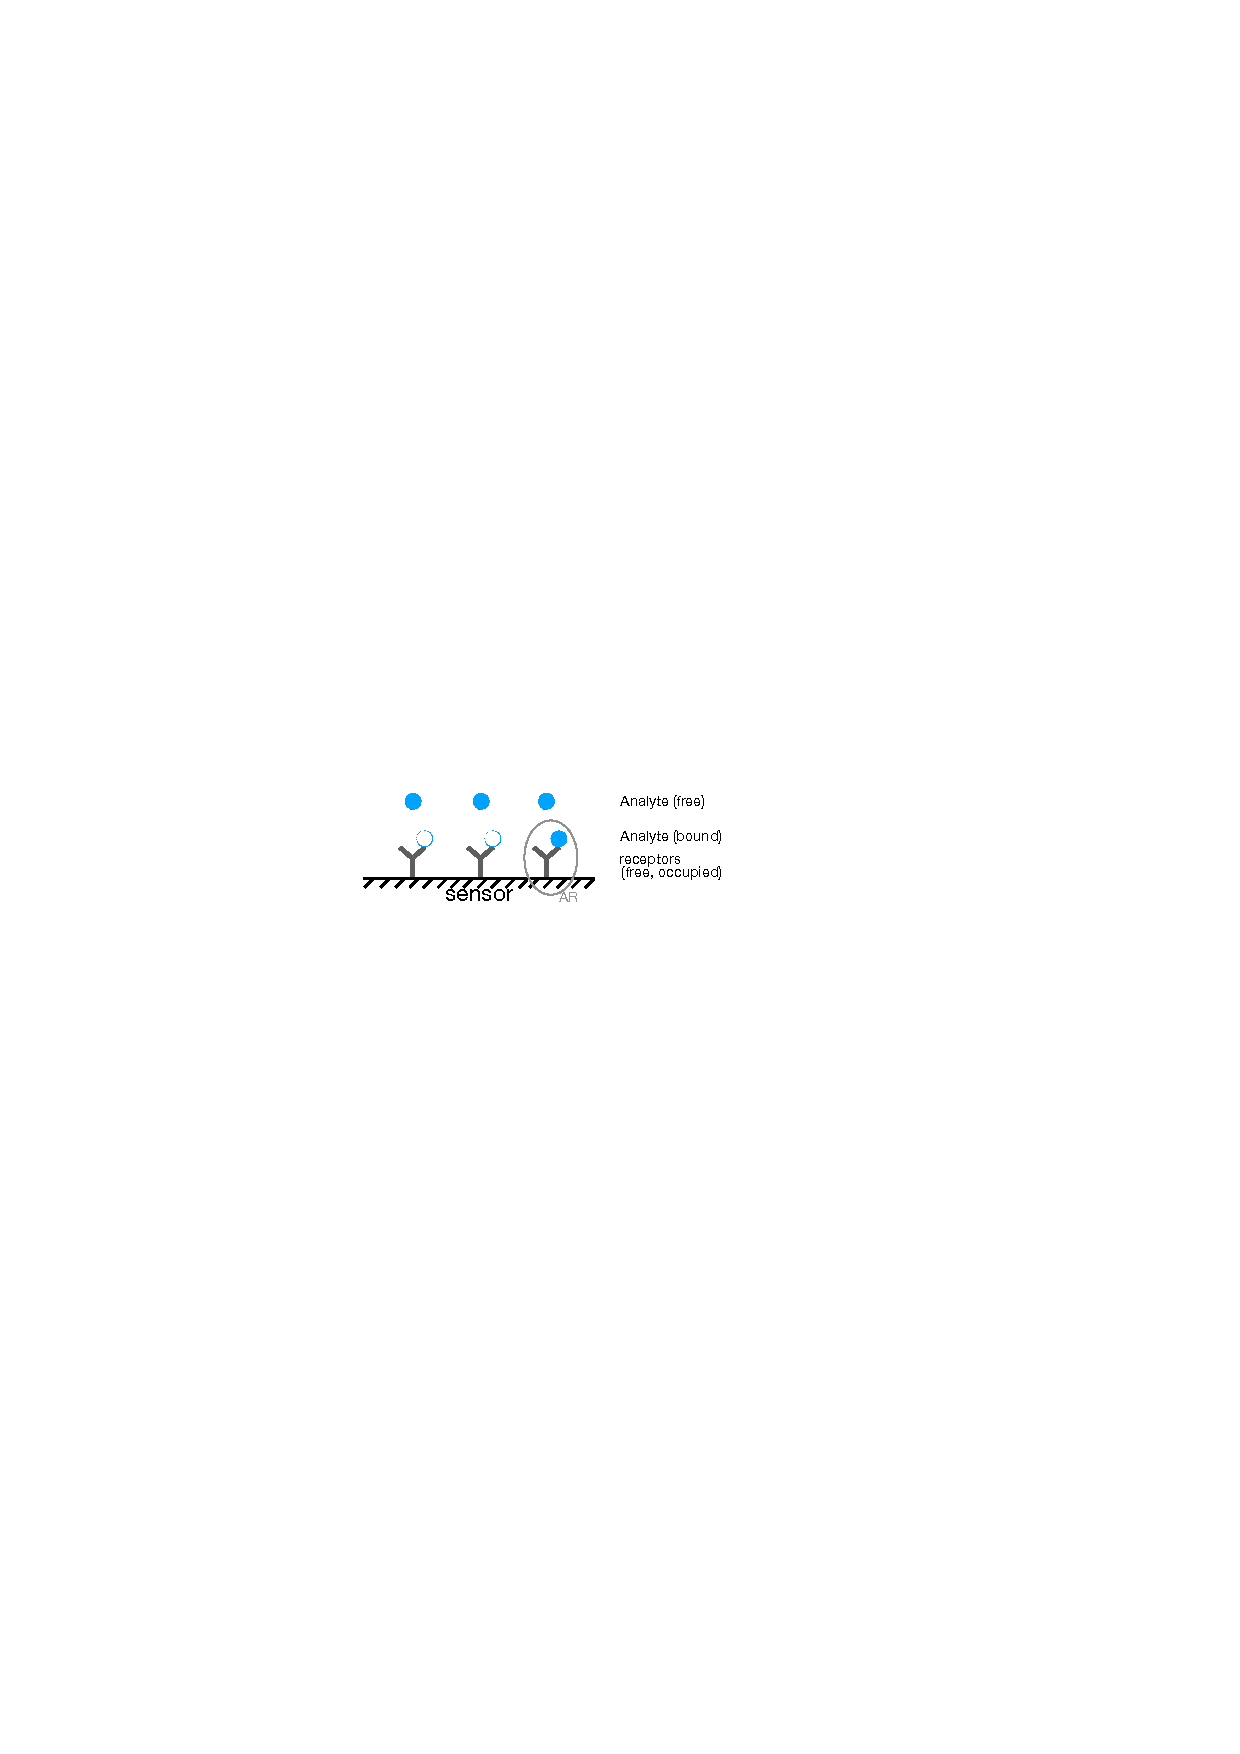
\includegraphics[width=.6\columnwidth]{Biosensors_Rules_of_Chemistry}
%%%%%%%%%%%%%%%%%%%%%%%%%%%%%%%%%%%%%%%%%%%%%%%%%%%%%%
\subsection{Sensitivity and Specificity}
%
%	All biosensing techniques are limited by the non-specific interaction = “It is not possible to catch \underline{only} Nemo with a fishing net”
%
\formula{Sensitivity}{\text{true positive rate (\% of correctly identified $+$)}}
\formula{Specificity}{\text{true negative rate (\% of correctly identified $-$)}}

Compensate Sensitivity through LOD.
%%%%%%%%%%%%%%%%%%%%%%%%%%%%%%%%%%%%%%%%%%%%%%%%%%%%%%
\subsubsection{Limit of Detection (LOD) \hfill \textnormal{(Sensitivity)}}
%
Limitation by non-specific binding (NSB) $\to$ noise at zero analyte

\begin{minipage}{.65\columnwidth}
    \formula{LOD}{LOD = 3\cdot\textrm{noise} / \deriv{S}{[A]}}
    \formbox{~}{S_{LOD} = S_0 + 3\cdot\textrm{noise}}
\end{minipage}%
\begin{minipage}{.35\columnwidth}
    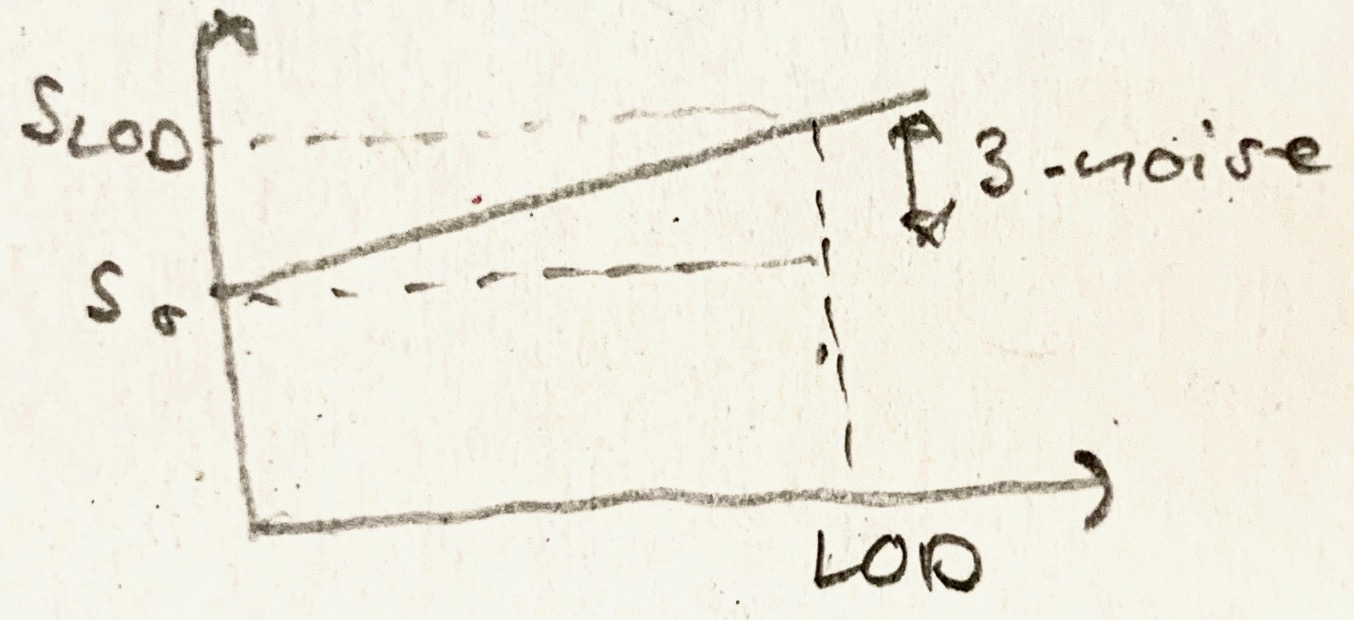
\includegraphics[width=\columnwidth]{Biosensors_LOD}
\end{minipage}

\formbox{LOD for intensity/signal}{LOD_{NSB} = \avg{I_{NSB}} + 3\;\sigma(I_{NSB})}
\formula{Lowest detectable intensity}{\frac{ \avg{I_{POI}} }{ LOD_{NSB} } = 1}
($\!\!~_{POI}$: proteins of interest)
\formula{Detectable \#proteins}{N\!\# = \frac{\Gamma}{m\ped{protein}}} \quad
$[\Gamma] = \unitfrac{pg}{mm^2}$ detection limit
